\documentclass[type=doctor]{thuthesis}
% 选项:
%   type=[bachelor|master|doctor|postdoctor], % 必选
%   secret,                                   % 可选
%   pifootnote,                               % 可选(建议打开)
%   openany|openright,                        % 可选,基本不用
%   arial,                                    % 可选,基本不用
%   arialtoc,                                 % 可选,基本不用
%   arialtitle                                % 可选,基本不用

% 所有其它可能用到的包都统一放到这里了,可以根据自己的实际添加或者删除。
\usepackage{thuthesis}

% 定义所有的图片文件在 figures 子目录下
\graphicspath{{figs/}}

% 可以在这里修改配置文件中的定义。导言区可以使用中文。
% \def\myname{薛瑞尼}

\begin{document}

%%% 封面部分
\frontmatter
%\thusetup{
%  %******************************
%  % 注意:
%  %   1. 配置里面不要出现空行
%  %   2. 不需要的配置信息可以删除
%  %******************************
%  %
%  %=====
%  % 秘级
%  %=====
%  secretlevel={秘密},
%  secretyear={10},
%  %
%  %=========
%  % 中文信息
%  %=========
%  ctitle={《高能物理中的数据分析》\\阅读笔记和习题解答},
%  cdegree={理学博士},
%  cdepartment={清华大学高能物理中心},
%  cmajor={高能物理实验},
%  cauthor={学生},
%  csupervisor={导师},
%  %cassosupervisor={陈文光教授}, % 副指导老师
%  %ccosupervisor={某某某教授}, % 联合指导老师
%  % 日期自动使用当前时间,若需指定按如下方式修改:
%  % cdate={超新星纪元},
%  %
%  % 博士后专有部分
%  %cfirstdiscipline={计算机科学与技术},
%  %cseconddiscipline={系统结构},
%  %postdoctordate={2009年7月——2011年7月},
%  %id={编号}, % 可以留空: id={},
%  %udc={UDC}, % 可以留空
%  %catalognumber={分类号}, % 可以留空
%  %
%  %=========
%  % 英文信息
%  %=========
%  etitle={Notes and Solutions to \\ \textit{Data Analysis in High Energy Physics}},
%  % 这块比较复杂,需要分情况讨论:
%  % 1. 学术型硕士
%  %    edegree:必须为Master of Arts或Master of Science(注意大小写)
%  %             “哲学、文学、历史学、法学、教育学、艺术学门类,公共管理学科
%  %              填写Master of Arts,其它填写Master of Science”
%  %    emajor:“获得一级学科授权的学科填写一级学科名称,其它填写二级学科名称”
%  % 2. 专业型硕士
%  %    edegree:“填写专业学位英文名称全称”
%  %    emajor:“工程硕士填写工程领域,其它专业学位不填写此项”
%  % 3. 学术型博士
%  %    edegree:Doctor of Philosophy(注意大小写)
%  %    emajor:“获得一级学科授权的学科填写一级学科名称,其它填写二级学科名称”
%  % 4. 专业型博士
%  %    edegree:“填写专业学位英文名称全称”
%  %    emajor:不填写此项
%  edegree={Doctor of Philosophy},
%  emajor={Experimental High Energy Physics},
%  eauthor={Students},
%  esupervisor={Professors},
%  %eassosupervisor={Chen Wenguang},
%  % 日期自动生成,若需指定按如下方式修改:
%  % edate={December, 2005}
%  %
%  % 关键词用“英文逗号”分割
%  ckeywords={},
%  ekeywords={}
%}

\begin{titlepage}
\centering
{\Large
%Tsinghua University\par
%Center for High Energy Physics\par
清华大学\par
高能物理中心\par
}
%\vfill
\vspace{18ex}
{\Huge\bfseries
《高能物理中的数据分析》\par 阅读笔记和习题解答\par
  %Peter Piper picked a peck of pickled peppers\par
}
\vspace{6ex}
{\Large
学习小组
\par}
\vfill
\parbox{.5\textwidth}{\centering 二〇一七年夏}
\end{titlepage}


% 如果使用授权说明扫描页,将可选参数中指定为扫描得到的 PDF 文件名,例如:
% \makecover[scan-auth.pdf]
%\makecover

%% 目录
\tableofcontents

%%引言
\chapter{序言}
\label{Preface}

在当今时代,随着科学研究对精确度、准确度要求的逐渐提高,统计推断在科研中正扮演着日益重要的角色。事实上,许多研究结果的获取,可以并且只能借助于复杂精妙的统计学手段。这一现象在高能物理实验领域当中体现的尤为明显,在我们的数据分析工作中,统计推断的知识无处不在。

近些年来,新的统计手段和以其为基础的复杂的软件工具如雨后春笋般地出现,这一方面为高能物理实验的数据分析工作提供了极大的便利,另一方面,其背后所隐含的复杂精巧的统计学原理则对实验人员的知识水平提出了更高的要求,这也是本书被撰写的目的所在——即为高能物理的从业人员提供统计推断方面的知识基础。本书面向的对象包括从学生到教授各个知识层面的研究人员,旨在对其高能物理数据分析上的工作提供全面而有具有可操作性的建议。为此,全书分为十二个章节,每个章节具有一个明确的主题,并由该方面的专家进行撰写,具体说明如下:

第一章里,我们将为读者介绍统计分析最为基本的概念,例如概率密度函数及其性质,常见的分布类型(高斯分布、泊松分布等),以及“概率”这一概念的两种不同含义——频率论述和贝叶斯论述。

接下来,我们将利用三个章节的篇幅,讲解如何利用统计学知识,从实验数据中提取各种信息: “参数估计”主要介绍如何通过拟合实验数据,得到模型参数的最优估计值,例如信号强度的估计等等;“假设检验”主要介绍如何评估某一假设正确与否,例如评估某一数据集究竟应该由已知本底的统计涨落来解释,还是其中真正包含了我们所关心的物理信号;“区间估计”则主要讨论如何给出参数的置信区间,例如信号强度的上限等。

在此之后,我们将对一些常见的话题进行更加深入的讨论。“分类”一章将会介绍数种不同的方法,以更好地进行事例区分,例如利用多变量分析的手段从本底样本中进行信号提取。这些方法往往能够非常有效地提高测量的灵敏程度,在某些情况下,能够借此观察到传统的事例区分方法下无法观测到的信号。“解谱法”一章中,我们将讨论在估计了各种系统偏差之后,如何对数据进行修正使之恢复原貌。这种方法在对微分分布的测量中具有较多的应用。"约束拟合"中,我们将说明如何在测量中引入物理定律所决定的约束条件,用来提高测量精度,或是估计未知的参量。

系统误差的估计往往是数据分析的最后一步,也往往是最关键的步骤之一。因此,在接下来的两个章节中,我们将着重介绍系统误差这一在其他教材中往往被忽视的话题。“如何处理不确定度”一章讲介绍如何估计各种来源的系统误差及其对最终结果的影响,以及如何避免这一影响。“理论不确定度”介绍了以强相互作用为代表的各种理论误差的处理方式。

行百里路者半九十。本书的最后三个章节,将为读者介绍这些统计学知识在实际的高能物理学中的具体应用。第十章,“高能物理领域常用的统计方法”,将为读者介绍多种在实践中常用的方法,如样本成分估计中常用的样板矩阵(卧槽这里怎么这么奇怪)法,以及用于估计分析过程导致的系统偏差的综合测试法。“分析实例”一章则主要列举了包含新粒子的寻找和新粒子性质测量在内的两个实际的物理分析,并以此为依托综述全书。最后一章“天文学中的应用”,将带领读者一探数据分析技巧在天文学中的巧妙应用。

在撰写各个章节的过程中,我们都尽可能地插入实例,以保证内容的实际、具体。通过完成每个章节后的习题,读者可以对本书中的材料有更加准确、深刻的理解。习题的提示和答案,以及一些必要的软件,都可以在出版社提供的网站上找到。此外,也欢迎读者们向本书的作者提供与本书相关的各类反馈。详情请访问www.wiley.com,屠龙宝刀,点击就送。

在此,我们要对在成书过程中提供帮助的团体和个人表示由衷的感谢。首先,要感谢每个章节的撰写者。其次,要感谢在编辑过程中参与讨论的大量同事们,但由于人数众多,篇幅所限,并不能一一列举:感谢Katarina Brock对图片的调整和排版;感谢来自Wiley的Konrad Kieling对本书的排版;感谢同样来自Wiley的Vera Palmer和Ulrike Werner在成书过程中的持续帮助。另外,还要感谢Tatsuya Nakada对我们使用他的习题材料的许可。

最后,真诚地感谢我们的朋友、伴侣和家人。没有你们的支持,这本书也将无法问世。


%% 符号对照表
\begin{denotation}[3cm]
\item[缩写] 全称
\end{denotation}



%%% 正文部分
\mainmatter
\chapter{基本概念}
\label{chap-fundamental}
  
\section{练习}
 % chap-fundamental
\chapter{参数估计}
\label{chap-parameter-estimation}
  
\section{练习}
 % chap-parameter-estimation
\chapter{假设检验}
\label{chap-hypothesis-testing}
  
\section{练习}
 % chap-hypothesis-testing
\chapter{区间估计}
\label{chap-interval-estimation}
  
\section{练习}
 % chap-interval-estimation
\chapter{分类}
\label{chap-classification}

\section{练习}
 % chap-classification
\chapter{解谱法}
\label{chap-unfoldin}
  
\section{练习}

 % chap-unfolding
\chapter{约束拟合}
\label{chap-constrained-fits}
  
\section{练习}
 % chap-constrained-fits
\chapter{如何处理系统不确定度}
\label{chap-systematic-uncertainties}
  
\section{练习}
 % chap-systematic-uncertainties
\chapter{理论不确定度}
\label{chap-theory-uncertainties}
  
\section{练习}
 % chap-theory-uncertainties
\chapter{高能物理领域常用的统计方法}
\label{chap-statistical-methods}
  
\section{练习}
 % chap-statistical-methods
\chapter{分析实例}
\label{chap-analysis}

\section{练习}
 % chap-analysis


%%% 其它部分
%\backmatter

%% 本科生要这几个索引,研究生不要。选择性留下。
% 插图索引
%\listoffigures
% 表格索引
%\listoftables
% 公式索引
%\listofequations


%% 参考文献
% 注意:至少需要引用一篇参考文献,否则下面两行可能引起编译错误。
% 如果不需要参考文献,请将下面两行删除或注释掉。
%\bibliographystyle{thuthesis-numerical}
%\bibliography{ref/refs}


%% 致谢
%\include{data/ack}

%% 附录
\begin{appendix}
%\input{data/appendix01}
\end{appendix}

%% 个人简历
%\include{data/resume}

%% 本科生进行格式审查是需要下面这个表格,答辩可能不需要。选择性留下。
% 综合论文训练记录表
%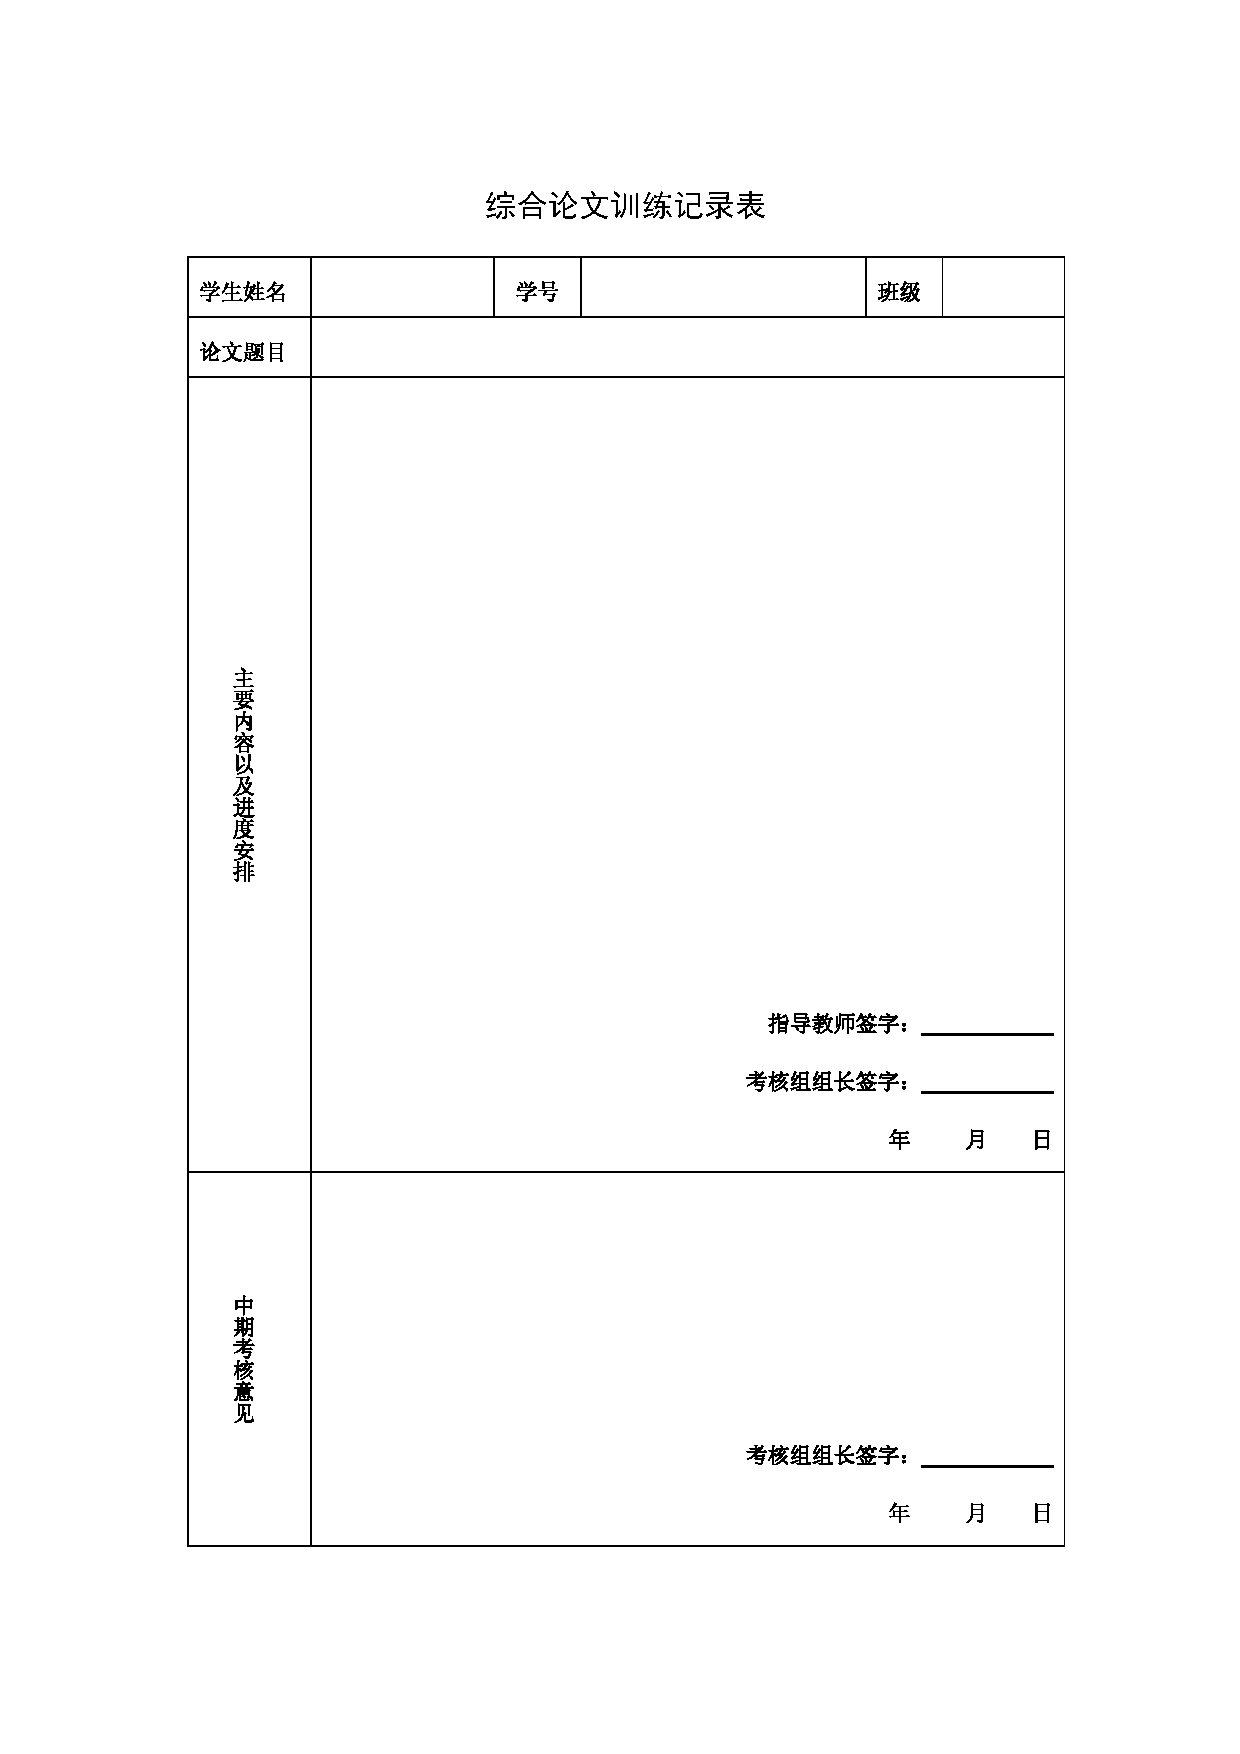
\includepdf[pages=-]{scan-record.pdf}
\end{document}
